\chapter{Video and Animation}
Video data can be generated in two different ways: 

\begin{itemize}
	\item by recording the real world and 
	\item through synthesis based on a description
\end{itemize}

\section{Basic Video Concepts}
The human eye is the human receptor for taking in still pictures and motion pictures. Its inherent properties determine, in conjunction with neuronal processing, some of the basic requirements underlying video systems.

\subsection{Video Signal Representation}
In conventional black-and-white television sets, the video signal is usually generated by means of a Cathode Ray Tube (CRT). An electron beam carries corresponding pattern information, such as intensity in a viewed scene.

The representation of a video signal comprises three aspects: 
\begin{itemize}
	\item visual representation
	\item transmission, and 
	\item digitization.
\end{itemize}
\subsubsection{Visual Representation} 
A key goal is to present the observer with as realistic as possible a representation of a scene. In order to achieve this goal, the television picture has to accurately convey the spatial and temporal content of the scene. Important measures for this are:


\begin{enumerate}
	\item \textit{Vertical details and viewing distance}
	
	The geometry of a television image is based on the ratio of the picture width $ W $ to the picture height $ H $. This width-to-height ratio is also called the aspect ratio. The	conventional aspect ratio (for television) is $ 4/3=1.33 $. Figure {\ref{fig:decomposition-of-motion-picture}} shows an
	example of this ratio.

%%%%%%%%%%%%%%%%%%%%%%%%%%%%%%%%%%%%%%%%%
%										%
%				FIGURE				   	%
%										%
%%%%%%%%%%%%%%%%%%%%%%%%%%%%%%%%%%%%%%%%%
\begin{figure}[h]
	\centering
	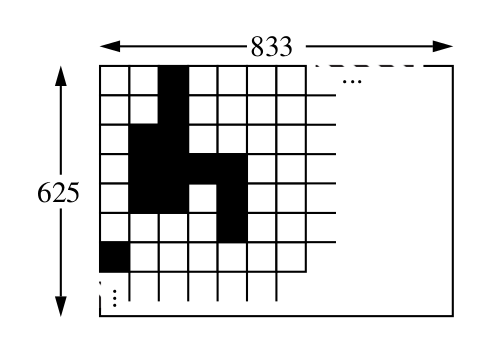
\includegraphics[width=0.8\textwidth]{decomposition-of-motion-picture}
	\caption{Decomposition of a motion picture.}{\label{fig:decomposition-of-motion-picture}}
\end{figure}
%--------------------------Figure end -------------------
The viewing distance $ D $ determines the angular field of view. This angle is usually calculated as the ratio of the viewing distance to the picture height ($ D/H $).

\item \textit{Horizontal detail and picture width}

The picture width normally used for television is $ (\frac{4}{3}  \times picture \:height )$ i.\ e.\ ($ 4/3 $ times the picture height). The horizontal field of view can be determined using the aspect ratio.

\item \textit{Total detail content of a picture}

The vertical resolution is equal to the number of picture elements of the picture height, while the number of horizontal picture elements is equal to the product of the vertical resolution and the aspect ratio. 

The product of the picture’s elements	vertically and horizontally is the total number of picture elements in the image. 

However, in the case of television pictures, not all lines (and columns) are visible to the observer. The invisible areas are often used to transmit additional information.

\item \textit{Depth perception}

In nature, humans perceive the third dimension, depth, by comparing the images perceived by each eye, which view from different angles. In a flat television picture, a considerable portion of depth perception is derived from the perspective appearance of the subject matter. 

Further, the choice of the focal length of the camera lens and changes in depth of focus influence depth perception.
	
\item \textit{Luminance and Chrominance}

Color perception is achieved by three signals, proportional to the relative intensities of \textit{red}, \textit{green}, and \textit{blue} light (RGB) present in each portion of the scene. These	are conveyed to the monitor separately and the tube reproduces them at each point in time (unlike a camera). Often a different signal division is used for transmission and storage: 
\begin{itemize}
	\item one brightness signal (luminance), and 
	\item two color difference signals (chrominance).
\end{itemize}


\item \textit{Temporal aspects of illumination}	 

This property is used in television, in films, and for video data in computer systems. The impression of motion is created by presenting a rapid succession of barely differing still pictures (frames). Between frames, the light is cut off briefly. 

Two conditions must be met in order to represent a visual reality through motion pictures.
\begin{itemize}
	\item First, the rate of repetition of the images must be high enough to ensure continuity of movements (smooth transition) from frame to frame. 
	\item Second, the rate must be high enough that the continuity of perception is not disrupted by the dark intervals between pictures.
\end{itemize}


\item \textit{Continuity of motion}

	It is known that continuous motion is only perceived as such if the frame rate is higher than 15 frames per second. To make motion appear smooth, at least 30 frames per second must be used if the scene is filmed by a camera and not generated synthetically.
		
\item \textit{Flicker}
	
	If the refresh rate is too low, a periodic fluctuation of the perceived brightness can result. This is called the flicker effect. The minimum refresh rate to avoid flicker is $ 50Hz $. Achieving continuous, flicker-free motion would thus require a high refresh rate. However, in both movies and television, there are technical measures	that allow lower refresh rates to be used.

\item \textit{Temporal aspect of video bandwidth}

	Temporal specification depends on the rate of the visual system to scan pixels, as well as on the human eye's scanning capabilities. From human visual perspective, the eye requires that a video frame be scanned every $ 1/25 $ second. This time is equivalent to the time during which a human eye does not see the flicker effect.
\end{enumerate}


\subsubsection{Transmission}
Video signals are often transmitted to the receiver over a single television channel. In order to encode color, consider the decomposition of a video signal into three subsignals. For reasons of transmission, a video signal is comprised of a luminance signal and two chrominance (color) signals. 


Several approaches to color encoding are described below.

\begin{itemize}
	\item \textit{RGB Signal}
	
	An RGB signal consists of separate signals for red, green, and blue. Every color can be encoded as a combination of these three primary colors. The values $ R $ (for red), $ G $ (for green), and $ B $ (for blue), are normalized such that white results when $ R+G+B = 1 $ in the normalized representation.
	
	\item \textit{YUV Signal}
	
	Since human vision is more sensitive to brightness than to color, a more suitable encoding separates the luminance from the chrominance (color information). Instead of separating colors, the brightness information (luminance $ Y $) is separated from the color information (two chrominance channels $ U $ and $ V $).⎄
	
	The YUV signal can be calculated as follows:
	\begin{align*}
	 	& Y = 0.30R + 0.59G + 0.11B  \\
	 	& U = (B-Y) \times 0.493  \\
		& V = (R-Y) \times 0.877&&
	\end{align*}

\item \textit{YIQ signal}

A similar encoding exists for NTSC’s YIQ signal:
	\begin{align*}
		& Y = 0.30R + 0.59G + 0.11B \\
		& I = 0.60R - 0.28G - 0.32B  \\
		& Q = 0.21R - 0.52G + 0.31B &&
	\end{align*}
\end{itemize}
\subsubsection*{Digitalization}
Before a motion picture can be processed by a computer or transmitted over a network, it must be converted from an analog to a digital representation.

This digitization process consists of the three steps of:
\begin{multicols}{3}
	\begin{enumerate}
		\item \textit{sampling},
		\item \textit{quantization}, and
		\item \textit{coding}.
	\end{enumerate}
\end{multicols}

In determining the sampling frequency, the \textbf{Nyquist Theorem} must be followed.
 
Nyquist theorem states that the signal being sampled cannot contain any frequency components that exceed half the sampling frequency. 

In order to prevent the base band from overlapping with repeating spectra and to allow for real hardware components not behaving ideally, the sampling rate is normally chosen somewhat higher than the limit dictated by the Nyquist Theorem.

Digitalization consists of sampling the gray (color) level in the picture at $ M \times N $ array of points. The next step in the creation of digital motion video is to digitize pictures in time and get a sequence of digital image per second for analog motion video.

Since the gray value of a sampled spot can take on any value in a continuous range, it must be quantized in order to be processed digitally. The gray-scale is subdivided into several ranges, and each pixel is assigned only one of these values.


\subsection{Computer Video Format}
The computer video format depends on the input and output devices for the motion video medium.

Current video digitalization hardware differs with respect to the resolution of the digital images (frames), quantization, and the frame rate (frames/second).

Motion video output depends on the display hardware used, usually a raster display. The typical architecture of such a device is shown in Figure {\ref{fig:raster-arch}}.


%%%%%%%%%%%%%%%%%%%%%%%%%%%%%%%%%%%%%%%%%
%										%
%				FIGURE				   	%
%										%
%%%%%%%%%%%%%%%%%%%%%%%%%%%%%%%%%%%%%%%%%
\begin{figure}[H]
	\centering
	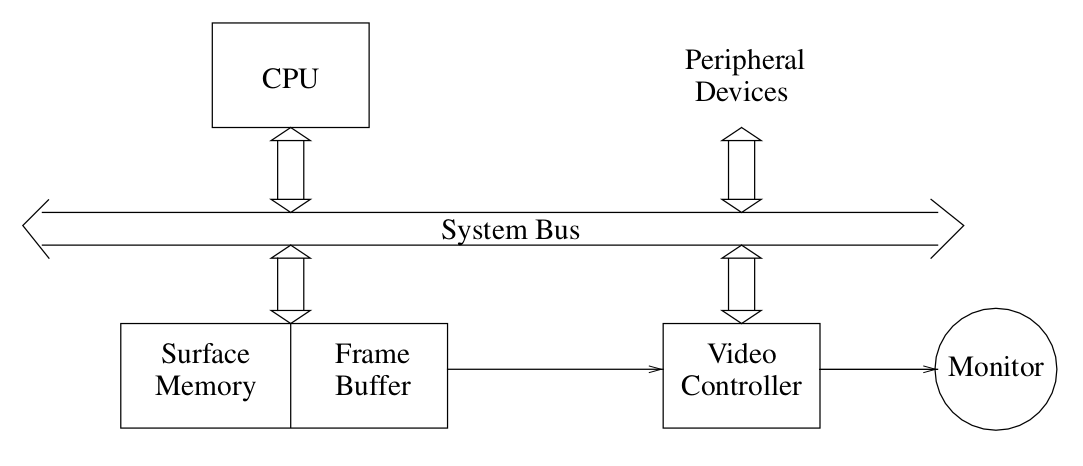
\includegraphics[width=0.8\textwidth]{raster-arch}
	\caption{Architecture of a raster display.}{\label{fig:raster-arch}}
\end{figure}
%--------------------------Figure end -------------------

\begin{itemize}
	\item The video controller displays the image stored in the frame buffer, accessing the buffer through a separate port as often as required by the video scanning rate. 
	\item The most important task is the constant refresh of the display. 
	\item Due to the disturbing flicker effect, the video controller cycles through the frame buffer, one scan line at a time, typically 60 times/second. 
	\item To display different colors on the screen, the system works with a Color Look-Up Table (CLUT or LUT). 
	\item At any given time, a limited number of colors ($ n $) are available for the whole picture. 
	\item The set of the $ n $ most frequently used colors is chosen from a color palette consisting of $ m $ colors, whereby in general  $n \ll m$.
\end{itemize}


Some computer video controller standards are given here as examples. Each of these systems supports different resolution and color presentation.

\begin{itemize}
	\item The \textit{Color Graphics Adapter (CGA)} has a resolution of $ 320 \times 200  $pixels with simultaneous presentation of four colors. Therefore, the storage capacity per image is:
	
	\begin{align*}
		320 \times 200 \: pixels \times \frac{2 \: bit/pixel}{8 \: bit/byte} = 16,000 \: bytes
	\end{align*}

\item The \textit{Enhanced Graphics Adapter (EGA)} supports display resolution of $ 640 \times 350 $ pixels with 16 simultaneous colors. The necessary storage capacity per frame is:

\begin{align*}
	640 \times 350 \: pixels \times \frac{4 \: bit/pixel}{8 \: bit/byte} = 1, 12,000 \: bytes
\end{align*}

\item The \textit{Video Graphics Array (VGA}) works mostly with a resolution of $ 640 \times 480 $ pixels with 256 simultaneous colors. The monitor is controlled via an analog RGB output. The necessary storage capacity per frame is:

\begin{align*}
	640 \times 480 \: pixels \times \frac{8 \: bit/pixel}{8 \: bit/byte} = 3, 07,200 \: bytes
\end{align*}

\item The \textit{Super Video Graphics Array (SVGA}) can present 256 colors at a resolution of $ 1,024 \times 768  $pixels. The necessary storage capacity per frame is:

\begin{align*}
	1,024 \times 768 \: pixels \times \frac{8 \: bit/pixel}{8 \: bit/byte} = 7,86,432 \: bytes
\end{align*}

Other SVGA modes include $ 1,280 \times 1,024 $ pixels and $ 1,600 \times 1,280 $ pixels.

\end{itemize}

\section{Animation}
To animate something is, literally, to bring it to life. An animation covers all changes that have a visual effect. Visual effects can be very different attributes: 

\begin{itemize}
	\item positions (\textit{motion dynamics}), form, color, transparency, structure, and 
	\item texture of an object (\textit{update dynamics}), as well as 
	\item changes in lighting, camera position, orientation, and focus.
\end{itemize}




Today, computer-based animations are produced, edited, and generated with the help of a computer using graphical tools to create visual effects. Naturally, the discipline of traditional, non-computer based animation continues to exist.

\subsection{Basic Concepts of Animation}

\subsubsection{Input Process}
\begin{itemize}
	\item Before the computer can be used, drawings must be digitized to create key frames.
	\item These digitized images can be produced by the computer using appropriate programs or created by digitizing photos or drawings. 
	\item The drawings may need to be carefully post-processed (e.\ g.\ , filtering) in order to clean up any glitches arising from	the input process.
\end{itemize}


\subsubsection{Composition Stage}
\begin{itemize}
	\item Individual frames in a completed animation are generated by using image composition techniques to combine foreground and background elements. 
\end{itemize}


\subsubsection{Inbetween Process}
\begin{itemize}
	\item The animation of movement from one position to another requires the composition of frames with intermediate positions (intermediate frames) between key frames.
	\item In computer-based animation, this in-between processing is done using interpolation methods. 
	\item In interpolation, the system obtains only the beginning and end positions. 
	\item Linear interpolation, sometimes called \textit{lerping}, is the simplest method.
	\item For example, if one uses lerping to calculate the intermediate positions of a ball that has been thrown in the air and uses only three key frames, as
	shown in Figure {\ref{fig:linear-interpolation}}(a), then the resulting motion of the ball, depicted in Figure {\ref{fig:linear-interpolation}}(b),
	is totally unrealistic.
\end{itemize}


%%%%%%%%%%%%%%%%%%%%%%%%%%%%%%%%%%%%%%%%%
%										%
%				FIGURE				   	%
%										%
%%%%%%%%%%%%%%%%%%%%%%%%%%%%%%%%%%%%%%%%%
\begin{figure}[H]
	\centering
	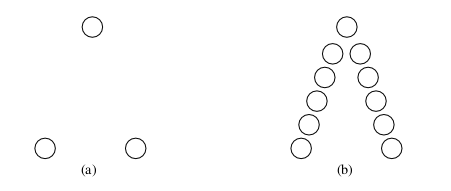
\includegraphics[width=0.8\textwidth]{linear-interpolation}
	\caption[Linear interpolation of the motion of a ball]{Linear interpolation of the motion of a ball: (a) key frames, (b) additional intermediate frames}{\label{fig:linear-interpolation}}
\end{figure}
%--------------------------Figure end -------------------

Due to the disadvantages of lerping, splines are often used to smooth out the interpolation between key frames. Splines can be used to smoothly vary different parameters as a function of time. With splines, individual points (or individual objects) can be moved in a natural fashion through space and time. 


\subsubsection{Changing Colors}
To process color changes, computer-based animation uses the Color Look-Up	Table (CLUT) or Look-Up Table (LUT). 
\begin{itemize}
	\item The animation is generated by manipulating the LUT.
	\item The simplest method is to cyclically change the colors of the LUT, thereby changing the colors of different parts of an image. 
	\item Performing LUT animation is relatively fast.
\end{itemize}

\subsection{Animation Languages}
Various languages exist to describe animations and new formal specification are currently being researched and further developed.

These specifications can be divided into the following three categories:

\subsubsection{Linear-List Notations}
In linear list notation each event in an animation is described by:
\begin{itemize}
	\item a beginning frame number, 
	\item an end frame number, and 
	\item an action (event) that is to be performed.
\end{itemize}

 Actions typically accept input parameters in the form of an instruction such as the following:
\begin{lstlisting}[numbers=none]
42, 53, B, ROTATE "PALM", 1, 30
\end{lstlisting}
This instruction means that between frames 42 and 53, the object denoted PALM should be rotated 30 degrees around axis 1. A table determines the rotation in each individual frame, allowing for animations with either uniform or accelerated movement.


\subsubsection{High-Level Programming Language Notations}
Another way to describe animations is by embedding animation control in a general-purpose programming language. The values of variables in the language can then be used as parameters for animation routines.

ASAS is an example of such a language based on an extension of LISP. The language’s primitives include vectors, colors, polygons, surfaces, groups, points of view, subworlds, and aspects of lighting. ASAS also includes a large collection of geometric transformations that operate on objects. 

The following ASAS program fragment describes an animated sequence in which an object called \textit{my-cube} is rotated while the camera pans. This fragment is evaluated for each frame in order to generate the entire sequence.


\begin{algorithm*}[H]
	(\textbf{grasp} my-cube); \textit{Make the cube the current object} \\
	
	(\textbf{cw} 0.05); \textit{Small clock-wise rotation} \\
	
	(\textbf{grasp} camera); \textit{Make the camera the current object} \\
	
	(\textbf{right} panning-speed); \textit{Move it to the right}
\end{algorithm*}


%\begin{lstlisting}
%(grasp my-cube); Make the cube the current object
%(cw 0.05); Small clock-wise rotation
%(grasp camera); Make the camera the current object
%(right panning-speed); Move it to the right
%\end{lstlisting}

\subsubsection{Graphical Languages} 
A problem with traditional, textual programming languages is that graphical actions cannot be easily visualized by examining scripts.
\begin{itemize}
	\item Graphical animation languages describe animations in a more visual fashion. 
	\item Such languages are used to name and edit the changes taking place simultaneously in an animation and to visualize the effects created. 
	\item The description of actions to be carried out is done using visual paradigms. 
	\item \textit{GENESYS}, \textit{DIAL} and the \textit{S-Dynamics System} are examples of such systems.
\end{itemize}

\subsection{Methods of Controlling Animation}
Animation control is independent of the language used to describe animation. There are various techniques for controlling animation.

\subsubsection{Full Explicit Control}
\begin{itemize}
	\item The simplest type of animation control. 
	\item The animator provides a description of all events that could occur in an animation. 
	\item This can be done by specifying simple transformations-such as \textit{scalings}, \textit{translations}, and \textit{rotations}-or by specifying key frames.
	\item An example of this type of control is the \textit{BBOP} system.
	\end{itemize}


\subsubsection{Procedural Control}
\begin{itemize}
	\item Procedural control is based on communication among different objects whereby each object obtains knowledge about the static or dynamic properties of other objects. \item This information can be used to verify that objects move consistently.
	\item In particular, in systems that represent physical processes, the position of an object can influence the movement of other objects (for example, ensuring that balls cannot move through walls). 
	\item In actor-based systems, individual actors can pass their positions along to others in order to influence their behavior.
\end{itemize}


\subsubsection{Constraint-Based Control}
Although some objects in the real world move along straight lines, this is not always the case. Many objects’ movements are determined by other objects with which they come in contact.
\begin{itemize}
	\item It is thus much simpler to specify an animation sequence using constraints instead of explicit control. 
	\item Sutherland's \textit{Sketchpad} and Borning's \textit{ThingLab} are examples of systems using constraints for control.
\end{itemize}


\subsubsection{Tracking Live Action}
By examining the motions of objects in the real world, one can animate the same movement by creating corresponding sequences of objects. Traditional animation uses \textit{rotoscoping}. 
\begin{itemize}

	\item A film is made in which people or animals act out the parts of the performers in the animation. 
	\item Afterwards, animators process the film, enhancing the background and replacing the human actors with the animated equivalents they have created.
	\item Another such technique is to attach indicators to key points on the body of a	human actor. 
	\item The coordinates of the corresponding key points in an animated model can be calculated by observing the position of these indicators.
	\item An example of this sort of interaction mechanism is the data glove, which measures the position and orientation of the wearer's hand, as well as the flexion and hyperextension of each finger point.
\end{itemize}


\subsubsection{Kinematic and Dynamic Control}

\subsubsection*{Kinematic Control}
\begin{itemize}
	\item Kinematics refers to the position and velocity of points. 
	\item A kinematic description of a scene, for example, might say, 
	\begin{quotation}
		\noindent ``The cube is at the origin at time $ t=0 $. Thereafter, it moves with constant acceleration in the direction ($ 1 \:meter, 1 \:meter, 5 \:meters $).''
	\end{quotation}

\end{itemize}

\subsubsection*{Dynamic Control}
 In contrast, dynamics takes into account the physical laws that govern kinematics (for example, the Newtonian laws for the movement of large bodies, or the Euler-Lagrange equations for fluids). 
\begin{itemize}
	\item particle moves with an acceleration proportional to the forces acting on it; the proportionality constant is the mass of the particle. 
	\item A	dynamic description of a scene might be: 
	\begin{quotation}
			\noindent ``At time $ t=0 $, the cube is at position  (\texttt{0 \:meter, 100 \:meter, 0 \:meter}). The cube has a mass of $ 100 \:grams $. The force of gravity acts on the cube.''
	\end{quotation}
	\item The natural reaction in a dynamic simulation is that the cube would fall.
\end{itemize}


\subsection{Display of Animation}\label{sec:animation_display}
\begin{itemize}
	\item To display animations with raster systems, the animated objects must be scan-converted and stored as a \textit{pixmap} in the frame buffer. 
	\item A rotating object can be shown by displaying successive views from slightly different locations.
	\item The scan-conversion must be done at least 10 (preferably 15 to 20) times per second in order to give a reasonably smooth visual effect; hence a new image must be generated in at most $ 100ms $. 
	\item The actual scan-conversion of an object should take only a small portion of this time otherwise distracting ghost effects appears.
	\item \textit{Double buffering} is used to avoid this (distracting ghost effects) problem. 
\end{itemize}

As an example, consider the display of a rotation animation. Assuming that the two halves of the pixmap are $ image_0 $ and $ image_1 $, the process is as follows:

  \begin{algorithm}[H]
  	 \texttt{Load LUT} to display values as background color \\
  	 \texttt{Scan-convert} object into $ image_0 $ \\
  	 \texttt{Load LUT }to display only $ image_0 $ \\
  	\textbf{Repeat} \\
  	
  \Indp 
  	\texttt{Scan-convert} object into $ image_1 $\\
  	\texttt{Load LUT} to display only $ image_1 $\\
  	\texttt{Rotate }object data structure description\\
  	\texttt{Scan-convert} object into $ image_0 $\\
  	\texttt{Load LUT} to display only $ image_0 $\\
  	\texttt{Rotate} object data structure description\\
  \Indm\textbf{Until} (termination condition)\\
\end{algorithm}

If rotating and scan-converting the object takes more than $ 100ms $, the animation is quite slow, but the transition from one image to the next appears to be instantaneous. Loading the LUT typically takes less than $ 1ms $.


\subsection{Transmission of Animation}
Animated objects can be represented symbolically using graphical objects or scan-converted pixmap images. Hence, the transmission of an animation may be performed using one of two approaches:

\subsubsection{Symbolic Representation}
The symbolic representation (e.g., circle) of an animation’s objects (e.\ g.\ , ball) is transmitted together with the operations performed on the object (e.\ g.\ , roll the ball). The receiver displays the animation as described earlier (see Section \ref{sec:animation_display}, Page No. \pageref{sec:animation_display}). Since the byte size of such a representation is much smaller than a pixmap representation, the transmission time is short. However, the display time is longer since the receiver must generate the corresponding pixmaps.

In this approach, the bandwidth (e.\ g.\ $ bytes/second $) required to transmit an animation depends on:
\begin{itemize}
	\item the size of the symbolic representation structure used to encode the animated object
	\item the size of the structure used to encode the operation command, and 	
	\item the number of animated objects and operation commands sent per second
\end{itemize}


\subsubsection{Pixmap Representation}
The pixmap representations of the animated objects are transmitted and displayed by the receiver. The transmission time is longer compared to the previous approach because of the size of the pixmap representation. However, the display time is shorter.

The necessary bandwidth is at least proportional to the size of a single pixmap	image and to the image repetition rate. These values are significantly higher than in the case of a symbolic representation.

\newpage\thispagestyle{empty}
